
Despite progress in recent years, reproducibility remains a challenge in recommender systems research \cite{beel2016towards}. Minor differences in parameters and experimental settings can yield incompatible results, which make it difficult to provide definitive answers about the relative properties of different algorithms. Progress in this area is supported by providing platforms on which comparative experiments can be conducted using declarative experimental configuration (so that experimental settings can be easily shared), with pre-implemented methodological workflows, and with a large library of algorithms for rapid benchmarking. 

In this section, I describe \libauto{}, an open-source command-line Python package providing a wrapper for the well-known LibRec 2.0 recommender systems algorithm library\footnote{www.librec.net}. My contributions to this project were the implementation and addition of in-processing and post-processing fairness algorithms and fairness metrics. The detail of each method is describe in the following section.

\subsection{Librec-auto}
% In \cite{mansoury2018automating}, we introduced \libauto{}, an open-source command-line Python package providing a wrapper for the LibRec 2.0 recommender systems algorithm library\footnote{www.librec.net}. 
This tool has been presented in \cite{mansoury2018automating} and provides an environment that supports automated experimentation. Therefore it supports reproducibility of research in recommendation algorithms.

Key advantages of \libauto{} were its ability to support typical research workflows, to offer a declaration configuration system, and to supplement experiment execution with the scripted production of human-friendly outputs including visualizations.

We have now extended this platform in a number of ways, particularly to support research in fairness-aware recommendation. \libauto{} now supports the current 3.0 version of the LibRec library and can take advantage of the new algorithms (including deep learning algorithms) found there. The \libauto{} project has also enhanced LibRec with a suite of metrics for measuring the fairness of recommendation outcomes. Most significantly, the tool now supports recommendation re-ranking, a common approach to enhancing fairness, diversity, and other non-accuracy properties of recommendation outcomes.

\subsubsection{\textbf{Core features}}
\hfill

LibRec 3.0 is a Java-based recommendation generation platform. It has been available to the recommender systems community since 2015 \cite{guo2015librec}, and has large library of implemented recommendation algorithms (more than 70 as of this writing). The platform supports a variety of evaluation metrics and evaluation methodologies. However, our experience indicates that for practical experimentation and reproducibility research, LibRec by itself is not sufficient. For example, intermediate computational outputs, such as recommendation results, cannot be reused as input for new evaluation metrics, requiring the re-execution of potentially lengthy experiment executions.

We developed \libauto{}\footnote{github.com/that-recsys-lab/librec-auto} to retain the benefits of working with LibRec while adding support for experimentation. A sketch of the functionality of \libauto{} is provided in Figure~\ref{fig:librec-auto}. As the figure indicates, LibRec is encapsulated and its various component elements are used to execute particular portions of the experimental workflow. In addition, the optional re-ranking component allows for the study of re-ranking algorithms not within the scope of LibRec's design. The key inputs are data and an XML-based configuration file. A particular study may consist of multiple experiments, all of which are configured at the same time in the configuration file. Configuration files are modular, so that, for example, multiple studies can share the same methodology elements, preventing inadvertent misconfiguration. 

Although the figure indicates a straight-line of execution, parallelism is built into \libauto{} at the level of experiment execution. Because experiments can have lengthy execution times, the post-processing phase allows for integration with messaging platforms, including Slack, so that experimenters are notified when their tasks are complete. These messages can include visualizations of experimental output, to provide a quick overview of results. 

\begin{figure}
    \centering
    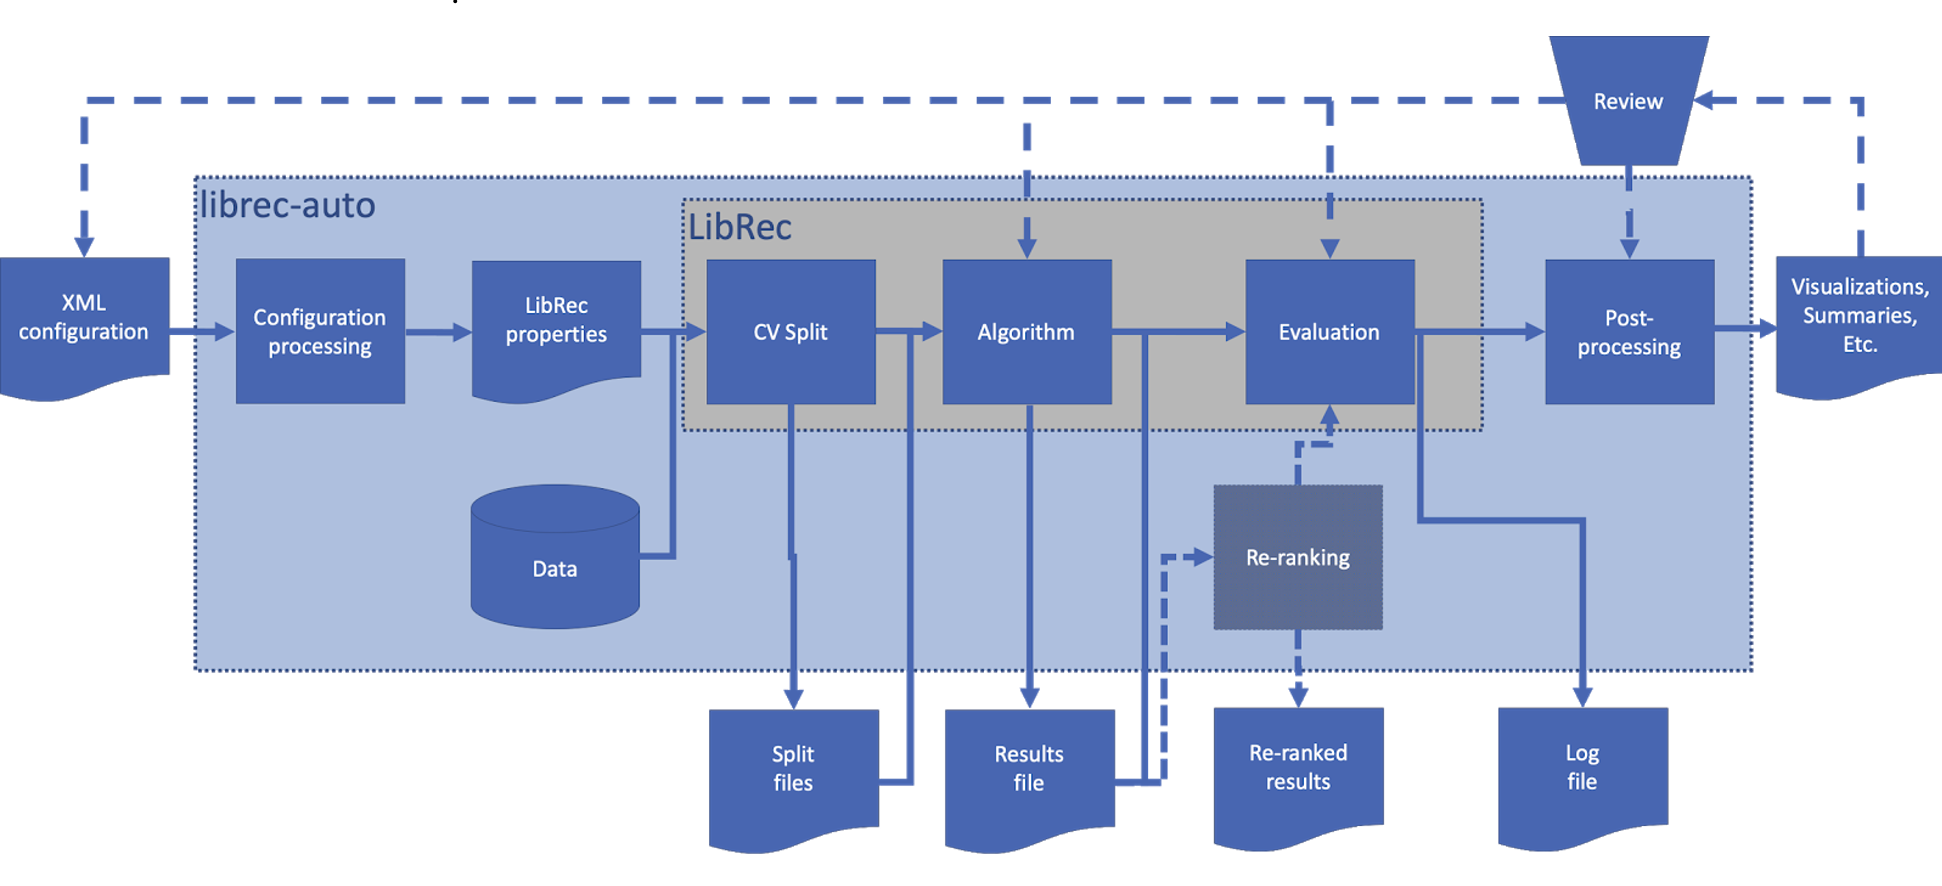
\includegraphics[width=5.25in]{imgs/la/librec-auto-diagram2.png}
    \caption{Schematic of experimentation workflow with \libauto{}. The LibRec library (Java, shown in grey) is encapsulated by \libauto{} (Python, shown in blue), which manages configuration, experimental outputs and post-processs. Added from \cite{mansoury2018automating} is the new re-ranking module shown in dark blue.}
    \label{fig:librec-auto}
    \vspace{-0.15in}
\end{figure}

\subsubsection{\textbf{Fairness-aware extensions}}
\hfill

Although \libauto{} has been under development since 2018, the latest release incorporates several key advances that specifically support common tasks in the study of recommendation fairness. These advances are (1) new evaluation metrics that report on fairness aspects of recommendation output, (2) an optional re-ranking step in the experiment pipeline, to support what is one of the most common category of fairness enhancing techniques, and (3) additional support for working with user (demographic) and item (content) features in algorithms and metrics. With these features, \libauto{} now can support a wide range of research activities in fairness-aware recommendation, and we will be adding additional capabilities in future releases.

Previously in the literature, many re-ranking algorithms have been proposed to achieve a balance between diversity and accuracy. The following methods try to achieve a fair representation between groups by penalizing the score of over-represented groups or reinforcing the score of the under-represented groups: (1) \textbf{FAR}, defined in \cite{liu2019farpfar}, combines a personalization-induced and fairness-induced scores with hyper-parameter $\lambda$; (2) \textbf{PFAR}, from \cite{liu2019farpfar}, adds a personalized weight to FAR, calculated based on item-features in user profile, representing the tolerance of the user for diverse resultsl and (3) \textbf{OFAiR} incorporates similar personalization and allows fine-grained control of protected group promotion when there are multiple protected groups \cite{sonboli2020opportunistic}. By contrast, (4) \textbf{FA*IR} \cite{zehlike2017fa} builds a queues of protected and unprotected items and draws from each queue to build the final re-ranked list. We also include two more general diversity-enhancing re-rankers first promoted in the information retrieval literature: (5) \textbf{MMR} diversifies result lists by greedily adding items with maximal marginal relevance \cite{carbonell1998use}, and (6) \textbf{XQuAD} defined in \cite{santos2010explicit} has similar goal to MMR algorithm, but it enhances diversity with respect to specific aspects. Finally, we include (7) \textbf{Calibrated Recommendations}, an algorithm closely tied to the Calibration metric above, which re-ranks recommendations to ensure a close match to the user's distribution of interests in item features~\cite{steck2018calibrated}. The re-ranking methods are part of \libauto{} and are implemented in Python.

Recommendation fairness and associated fairness metrics can be defined from the perspective of two main stakeholders: providers and consumers \cite{burke2017multisided}. Additionally, both provider-side and consumer-side metrics come in two basic varieties: exposure-based and hit-based. \textit{Exposure} metrics focus on the the appearance of protected items \cite{singh2018fairness} in a ranked list and \textit{hit-based} metrics take into account the suitability of the target user \cite{abdollahpouri2020multistakeholder}. Many metrics have been offered to measure recommendation fairness \cite{tsintzou2018bias,steck2018calibrated,beutel2019fairness,yao2017beyond,biega2018equity,castillo2019fairness,kuhlman2019fare,yang2017measuring}. We implement the following metrics in \libauto{} and where possible, both consumer-side and item-side versions of the metric are available: (1) \textbf{Discounted Proportional Fairness} (DPF), a hit-based fairness metric similar to the metric offered in \cite{castillo2019fairness} where it measures the ranking utility (nDCG) of the protected group with respect to the other groups. (2) \textbf{Calibration} \cite{steck2018calibrated}, a distribution-based metric that uses KL-Divergence to measure the difference in item category distribution between the preferences of users and their respective recommendation lists. (3) \textbf{Statistical parity}, based on the ideas discussed in \cite{zemel2013learning,ritov2017conditional}, measuring the difference in outcomes between protected and unprotected groups relative to various recommendation outcomes. Both ranking and prediction accuracy measures are supported. (4) \textbf{P-Percent-Rule} (PPR) discussed in \cite{biddle2006adverse}, is a two-sided extension of statistical parity \cite{barocas2016big}. (5) \textbf{Error-based} metrics proposed in Yao et al. \cite{yao2017beyond} including value-unfairness, absolute unfairness, underestimation unfairness, overestimation unfairness, and non-parity unfairness by Kamishima et al. \cite{kamishima2011fairness}. Additionally, we offer the following diversity-based metrics (6) \textbf{Intra-list distance (ILD)} \cite{ziegler2005improving}, a pairwise distance between all the item features in each user’s recommendation list, and (7) \textbf{Gini Index} calculated over the exposure of all the present groups in the recommendation list. All metrics are implemented in Java and integrated with the LibRec code base.

We plan future releases of \libauto{} to include integration with additional recommendation libraries, including LKPY~\cite{ekstrand2018lkpy}, LibFM~\cite{rendle2012factorization}, and DeepRec~\cite{zhang2019deeprec}.